\chapter{Customizing an existing Geocoder for the Twitter Domain}\label{chap2}

\section{Background: Geocoding Twitter}
Geocoding is the process of converting a human-readable location string into a pair of (latitude, longitude) coordinates. Human language is complex, which makes an excellent geocoding service a non-trivial task. For this reason, geocoding is typically done via a public search engine API service through Google, Bing, Yahoo, and others. The issue explored is whether the geocoders, trained to support search engine queries, can be used in the social media domain. 

Social media is a different domain from search engine queries. On social media, users are mindful of their privacy and hence are not likely to disclose their exact address. Search engine queries, on the other hand, are not visible to the world and users are not afraid to use specific keywords in order to get to the specific business or organization %such as for reading reviews about a specific business or getting to the business location.
(in order to get directions or find additional info). The issue is that while there are off-the-shelf commercial geocoders developed by search engine providers such as Google, there is no alternative developed specifically for social media. Many researchers utilize Google's geocoder despite it being not in Twitter's domain. Our research shows that we can improve Google's geocoder by identifying and removing geocoding errors on about a third of self-reported locations from Twitter.

Researchers that utilize commercial off-the-shelf geocoders typically report minimal preprocessing, if any. Preprocessing usually focuses on the query location itself. Preprocessing involves removing locations that are too broad (such as those with only state name), removing unnecessary punctuation, and auto-correcting any spelling errors. Our research highlights additional errors that may stem from the geocoder even for well-formed queries. For example, in the context of social media, a location such as `New York, New York' is most likely referring to New York City. Google's geocoder may associate the same query with the address of `New York New York Casino' located in Las Vegas, NV. In the context of a search engine query, the users that chose to spell out `New York, New York' must have had a higher click-through rate when a casino comes up vs. New York City. For a user utilizing Google Maps, it is not uncommon to search for a business name and expect a street level address match. In the context of social media, however, most users will post locations that are not indicative of a street level address. Social media locations are thus a different domain than the search engine queries that Google's geocoder expects. In this way, a lot of ambiguous queries such as `nowhere', `worldwide', and `my house' will produce coordinates to a matching street-level business address. There are additional caveats that Google's geocoder may take into account such as the IP from where the query is being performed. Thus for the same query, a researcher on the east coast might get different hits than a west coast researcher. 

Completely getting away from commercial off-the-shelf geocoders and writing custom rules for associating locations is not trivial. For example, rules that force both city and state name will miss well-known cities that are mentioned without a state. Focusing only on city name will cause issues for city names that appear across multiple states. Cities with long names will get missed due to misspelling or popular abbreviations. As a result, we do not recommend writing a solution from scratch, instead, an existing solution can be customized. 

Our research explores additional criteria, in the context of Twitter, that can be used to give greater confidence in the output of Google's geocoder. Locations with errors are identified by comparing the coordinates from users' messages to the geocoded coordinates from the self-reported location. We illustrate that a lot of these errors are associated with street level address associations (which should not be a common self-reported location on Twitter). Google's geocoder produces additional info such as the matching address components that can be used to rid of these errors. Incorporating our suggestions can %have significant ramifications on 
improve geocoding results and have an impact on studies related to population demographics, user's spatial proximity, and other use cases that utilize geocoders for processing Twitter users' self-reported locations.

\section{Related Research}

There are three types of Twitter-related locations: user home location, tweet location, and mentioned location [1]. Our focus was on home location which comes from the self-reported location field in the user's profile. This field can be available for more than 45\% of the underlying users [2]. Having it for a large sample of Twitter population, makes it suitable for analyzing population demographics [3], user's spatial proximity [4], election polls [5], and flu affected areas [6].

To be useful, each self-reported location needs to be converted to latitude and longitude. To convert the location information to coordinates, researches often rely on a single geocoding service such as Google [3, 5] or a combination of services such as through Bing, Google, and Yahoo when all report coordinates within X miles of each other [2, 4]. Other researchers completely get away from search engine geocoding APIs and utilize datasets such as GeoNames [7, 8] and custom parsers to match on the city and state names [6, 9]. 

The issue with the self-reported location field is that it can be anything, from being utterly blank to stating ambiguous or irrelevant information, such as `Planet Earth' [2, 14]. Basic preprocessing involves removing locations that are too vague (for example only state name) and removing ambiguous names via hand curated dictionaries (for example `Earth') [3, 4]. More advanced preprocessing involves breaking the string into address components, fixing each component for misspelling, abbreviation, and incorrect address format [10]. 

For validation of geocoder, coordinates of the self-reported location get compared against the central location in user's messages. Typically users with messages that contain GPS coordinates are utilized. The coordinates are aggregated across a user's tweets where the most frequent city or the geometric median serves as the user's home location [1]. Researchers have reported that the user's home location from the self-reported field does not correlate well to the location inferred from tweets [2, 11]. It has been argued that the user-declared profile locations differ from the physical locations that are being tweeted from and hence cannot be used as useful proxies for the physical locations [2]. This is due to both the self-reported location having erroneous or incomplete information [11] and due to tweets that contain coordinates irrelevant to the user's home address such as coordinates traveled to [12].

Self-declared locations have also been reported to have a poor correlation against the expected population distribution. Researchers used user-declared profile location as a query to Google Maps API, aggregated the returned locations into U.S. counties, and compared against 2000 US census data. Their findings showed that the Twitter population is a highly non-uniform sample of the population with mid-west significantly underrepresented and more populous counties consistently oversampled [3].

However, there is evidence that the online communities do correlate to the network we would expect from looking at the geographic proximity. For example, researchers used network density and social distance to show that smaller networks are more socially clustered and extend a smaller physical distance [4]. A more recent paper illustrated that spatial proximity and geographic factors do affect online social interactions [15]. 

We measured the discrepancy between Twitter users' self-declared locations and their actual physical locations for different location types. Existing research attempts to fix geocoding errors solely by fixing issues in self-reported location [2, 10]. While geocoding services themselves are typically tested in geocoding precise street-level addresses such as for locating specific restaurants [16]. In our study, we utilize the popular geocoder by Google and illustrate that some of the errors are due to the geocoder itself in that it attempts to match not only on geographic names but also on establishment and business name. 

Regardless of whether the error is stemming from poor geocoding or an ambiguous self-reported location, we illustrate that these errors can be identified and removed via additional parameters from the geocoder itself. Results illustrate reduced error between geocoded coordinates and the home location inferred from user's tweets. 

\section{Data}
Our data consisted of 1,038,826 Twitter users with 131,925 unique nonempty self-reported locations. Each user had a self-declared location that Google geocoded to the contiguous US and whose tweets contained either single point coordinate (coordinate geo-tag) or coordinates forming a bounding box (place-tag). Coordinate geo-tag was available for 491,365 users. 

It was important to consider place-tag because it recently became the default policy for associating geographic information with a tweet. The change, intended to reduce accidental privacy leaks, resulted in a significant drop in tweets with coordinate geo-tag [13]. Place-tag was used if it contained bounding box coordinates which were transformed into a single point at the center. 

For geocoding, we utilized a Python implementation for Google Maps Geocoding V3 API\footnote{https://developers.google.com/maps/documentation/geocoding}. Google allowed a maximum of 2500 queries per 24 hours so the geocoding results were collected over many weeks. Geocoder's region was set to `US' and language to `EN'. Table 2.1 shows additional output parameters from geocoder that were used in our research. 

\begin{table}
\small
\renewcommand{\arraystretch}{1.2}
\caption{Google Geocoder Output Parameters}
\label{table_ch2_1}
\centering
\begin{tabular}{|c|c|}
\hline
\bfseries Parameter & \bfseries Value\\
\hline
coordinates & latitude, longitude associated with the query\\
\hline
address & Each component consists of the component type, short name, \\
components & and long name. Example types are country, ADM1 (state), \\
& ADM2 (county), locality (city), street number, route, \\
& neighborhood name, postal code, and others. \\
 \hline
formatted &	Full address matched by Google, may not include all of \\
address & the address components (for example county usually omitted). \\
 \hline
address & Describes what the address is associated with, example values: \\
type & point of interest, university, restaurant, and others. \\
\hline
\end{tabular}
\end{table}

\section{Approach for Improving Geocoding}

The additional features from Table 2.1 were used to categorize self-declared locations that are associated with a low-level street address vs. a higher typically city-level location. As an example, Table 2.2 shows the output for query `New York, New York'. 

\begin{table}
\small
\renewcommand{\arraystretch}{1.2}
\caption{Google Geocoder Output for query `New York, New York'}
\label{table_ch2_2}
\centering
\begin{tabular}{|c|c|}
\hline
\bfseries Parameter & \bfseries Value\\
\hline
coordinates & lat: 36.1023715, lng: -115.1745559\\
\hline
address & street\_number: 3790, route: South Las Vegas Boulevard\\
component & locality: Las Vegas, ADM2: Clark County, ADM1:\\
type & Nevada, country: United States, postal\_code: 89109\\
\hline
Formatted & 3790 S Las Vegas Blvd, Las Vegas, NV 89109, USA\\
Address &\\
\hline
address type & casino, establishment, lodging, point\_of\_interest\\
\hline
\end{tabular}
\end{table}

From Table 2.2, casino, lodging, and establishment address types, as well as the street number in address components, are indicative of an address that is a street level address. Across all of the locations in our dataset, there were a total of 73 unique address components and 116 unique address types.

Table 2.3 shows the top 10 address components and address types that account for the biggest ratio of all locations. From the table, the address types of store, food, and restaurant are low-level locations that are not right to associate with most Twitter users.

\begin{table}
\small
\renewcommand{\arraystretch}{1.2}
\caption{Top 10 Most Frequent Address Type and Component}
\label{table_ch2_3}
\centering
\begin{tabular}{|c|c|c|c|}
\hline
\bfseries Address Type & \bfseries Ratio & \bfseries Address Component & \bfseries Ratio \\
\hline
political&0.6298&country&1\\
\hline
locality&0.566&administrative\_area\_level\_1&1\\
\hline
establishment&0.3101&locality&0.9639\\
\hline
point\_of\_interest&0.3068&administrative\_area\_level\_2&0.9481\\
\hline
store&0.0563&postal\_code&0.5652\\
\hline
food&0.0511&route&0.3348\\
\hline
neighborhood&0.04&street\_number&0.3027\\
\hline
restaurant&0.0395&administrative\_area\_level\_3&0.2005\\
\hline
university&0.0249&neighborhood&0.1827\\
\hline
route&0.0246&postal\_code\_suffix&0.1308\\
\hline
\end{tabular}
\end{table}

We developed a heuristic from these additional address attributes. According to our heuristic, a high-level location needs to have one or more of these attributes: political address type without a street number address component, postal code address type, or university address type.

The political address type refers to recognized divisions of a physical territory; locality, neighborhood, colloquial area, sub-locality, and other address types are part of it. Postal code and university are not of political type, but are considered to be reasonable locations for Twitter users to associate themselves with. In this way a location with one or more of these attributes is classified as a high-level location; otherwise, it is classified as low-level.

Out of 131,925 self-reported locations in our dataset our heuristic classified 46,091 as low-level and 85,834 as high-level. The next sections illustrate that the low-level locations carry a high error rate. Most of the low-level locations are impossible to geocode being generic keywords that Google's geocoder attempts to associate with a business name. Dataset can be improved by filtering out users whose self-reported location maps to a low-level address.

\section{Evaluation Methodology}

We refer to the home location from coordinates in tweets as Tweet-based Home Location (THL) and the geocoded self-reported location in the user's profile as Self-reported Home Location (SHL). THL was computed, for each user, using a geometric median over user's tweets containing coordinate geo-tags and place-tags.

In our study, the error for each user u is the distance in miles between THL and SHL:

\begin{equation}
ED(u) = distance(THL(u), SHL(u))
\end{equation}

where distance is computed using Vincenty's formula [17], it is more accurate than Euclidean distance because it considers the earth surface's curve.

Three popular measures are used to measure the overall error across users [18]; the mean, median, and the proportion of users with error under 100 miles:

\begin{equation}
MeanED = \frac{1}{|U|}\sum_{u \epsilon U}\ ED(u)
\end{equation}

\begin{equation}
MedianED = median_{u \epsilon U}\{ED(u)\}
\end{equation}

\begin{equation}
ACC@100 = \frac{|\{u \epsilon U|ED(u)\leq 100\}|}{|U|}
\end{equation}

where U represents the set of users of interest. Each measure is computed in miles. Note that higher values are better for $ACC@100$ while lower values are better for mean and median ED.

The subset of users can correspond to those users that utilize a specific location and can thus be used to compare error rates over various locations. Of particular interest was the error rate over users whose location maps to a high-level address type vs. other locations.

\section{Results}

The heuristic, described in the approach section, used additional geocoder output to label each location as high or low level. Our dataset consisted of 131,925 self-reported locations out of which 85,834 mapped to high-level and 46,091 mapped to low-level location type. Each error measure is computed for each self-reported location over all users that utilize it. For each location type, the average and standard deviation of error are computed over all self-reported locations that belong to the location type. Table 2.4 shows the average and standard deviation of error for low and high location types. The last two rows show the expected worst error rate for impossible to geocode locations. This is followed by the expected best error rate for accurately geocoded locations (as computed in the next two subsections). 

\begin{table}
\small
\renewcommand{\arraystretch}{1.2}
\caption{Error Rate for Each Location Type}
\label{table_ch2_4}
\centering
\begin{tabular}{|c|c|c|c|}
\hline
\bfseries Result Type & \bfseries MeanED & \bfseries MedianED & \bfseries ACC@100\\
\hline
Low level&1343.12+/-1938.5&1313.93+/-1940.91&0.28+/-0.44\\
\hline
High Level&227.34+/-782.5&195.33+/-778.96&0.78+/-0.37\\
\hline
Expected Worst&2657.75+/-1334.2&1968.74+/-1787.29&0.016+/-0.019\\
\hline
Expected Best&205.1+/-85.29&9.94+/-25.68&0.82+/-0.07\\
\hline
\end{tabular}
\end{table}

$ACC@100$ measure in table shows that self-reported Twitter locations that map to a low-level location type are confirmed by tweets for only 28\% of users; high-level locations are confirmed by 78\% of users. Mean and median error is also significantly higher for low-level location type. By cleansing the dataset from users whose self-reported location maps to a low-level location type will produce results that are more aligned to the best expected results, having $ACC@100$ of 82\%. Furthermore, the self-reported locations mapping to low-level location type are utilized by a small subset of users: the 46,091 low-level locations are used by only 103,270 out of 1,038,826 users.

The next sections will analyze specific locations in more detail. Subsection 2.6.1 utilizes manually verified properly geocoded locations for computing the expected best error rate. Subsection 2.6.2 utilizes locations that are impossible to geocode for computing the expected worst error rate. Subsection 2.6.3 attempts to categorize locations based on the $ACC@100$, the number of users, and expected error rates. Finally, subsection 2.6.4 analyzes popular locations with high and low error rates. 

\subsection{Accurately Geocoded Location Expected Error Rate}

Each error measure was computed over the top one-hundred most frequent locations, that were accurately geocoded, and used to compute the expected error rate. The average and standard deviation over the one-hundred locations are shown in the last row of table 2.4. Thus given a location that is accurately geocoded we expect a range of 75-89\% of users having their THL be within 100 miles of the geocoded coordinates. This represents the best possible error rate we expect to achieve since these were calculated over locations verified by hand and used by many users. Table 2.5 shows a sample of locations over which this error rate was computed. Each location in table 2.5 was accurately geocoded, but the coordinates in some user's messages don't confirm it. This is because some of the coordinates may be from places visited that are far from the user's real home location. 

\begin{table}
\small
\renewcommand{\arraystretch}{1.2}
\caption{ Sample Error for Accurately Geocoded Locations}
\label{table_ch2_5}
\centering
\begin{tabular}{|c|c|c|c|c|}
\hline
\bfseries Location & \bfseries Users & \bfseries MeanED & \bfseries MedianED & \bfseries ACC@100\\
\hline
Los Angeles, CA&22431&436.21&9.89&0.79\\
\hline
New York, NY&15375&344.08&5.08&0.81\\
\hline
Chicago, IL&13788&229.53&6.11&0.81\\
\hline
Houston, TX&11676&186.95&7.09&0.83\\
\hline
Los Angeles&11380&302.02&9.89&0.86\\
\hline
Washington, DC&10500&300.96&1.48&0.8\\
\hline
\end{tabular}
\end{table}

\subsection{Impossible to Geocode Location Expected Error Rate}
Similar to the previous subsection, here we investigate top locations that do not refer to a geographical area and thus cannot be geocoded accurately. Table 2.6 shows a sample of such locations. 

\begin{table}
\small
\renewcommand{\arraystretch}{1.2}
\caption{Sample Error for Impossible to Geocode Locations}
\label{table_ch2_6}
\centering
\begin{tabular}{|c|c|c|c|c|}
\hline
\bfseries Location & \bfseries Users & \bfseries MeanED & \bfseries MedianED \bfseries & \bfseries ACC@100\\
\hline
Earth&3125&3065.99&1308.67&0.00352\\
\hline
Worldwide&1277&2583.70&1231.46&0.00235\\
\hline
Everywhere&1042&1986.65&1251.54&0.02303\\
\hline
Global&850&2353.39&1229.36&0.03412\\
\hline
Planet Earth&722&2342.93&1544.00&0.0277\\
\hline
Hogwarts&574&3385.79&2141.28&0.01568\\
\hline
\end{tabular}
\end{table}

These locations were not used by as many users and as a result, the top fifty such locations were utilized when computing the expected error rate. Each location was used by at least one-hundred users. Three error measures were computed over users for each location and used to compute the average and standard deviation as shown in the second to last row of table 2.6. Thus for an inaccurately geocoded location, we expect 0-3.5\% of users to have their THL be within 100 miles of the geocoded coordinates. The only reason that the associated $ACC@100$ is not zero is that occasionally, as a matter of chance, such locations may match an establishment name whose address happens to be within a 100-mile radius of location from tweets. 

\subsection{Categorizing Locations using Error Rates}

Looking at the $ACC@100$, the number of users, and expected error rates allowed us to look at specific locations more closely and categorize them into four categories. $ACC@100$ calculates the percent of users whose tweets confirm the geocoded address. It is crucial to consider the number of users because as more users utilize the location, there is a corresponding increase in confidence for $ACC@100$. The expected best and expected worst error rates give us the $ACC@100$ range for how an accurately vs. inaccurately geocoded location is expected to behave. As a reminder for $ACC@100$, the worst expected rate was 0.015 +/- 0.019, and the best-expected error was 0.82 +/- 0.07. Thus on average 15 out of 1000 vs. 820 out of 1000 users will be in agreement for improperly and accurately geocoded locations, respectively. An example of each location category is shown in Table 2.7.

\begin{table}
\small
\renewcommand{\arraystretch}{1.2}
\caption{Location Category Examples}
\label{table_ch2_7}
\centering
\begin{tabular}{|c|c|c|c|}
\hline
\bfseries C & \bfseries Location to Google Mapping & \bfseries Users & \bfseries ACC@100\\
\hline
1&Los Angeles, CA to&22431&0.79484\\
&Los Angeles, CA, USA& & \\
\hline
2&Earth to 15612 S Keeler Terrace,&3125&0.00352\\
&Olathe, KS 66062, USA& & \\
\hline
3&New York, USA to New York, NY, USA&9010&0.57469\\
\hline
3&Disneyland to 1313 Disneyland Dr,&168&0.58333\\
&Anaheim, CA 92802, USA& & \\
\hline
4&Ocean Drive Miami, FL to&1&0\\
&Ocean Dr, Miami Beach, FL 33139, USA& & \\
\hline
4&Somewhere, Fishing to 1305 Snell Isle&1&1\\
&Blvd NE, St. Petersburg, FL 33704, USA& & \\
\hline
\end{tabular}
\end{table}

\begin{itemize}
\item Category 1: high $ACC@100$ ($\geq$0.75 using lower bound of expected best result) and many users. Generally, it is a well-formed self-declared location that is accurately geocoded. Example: `New York, NY'.  

\item Category 2: low $ACC@100$ ($\leq$0.034 using upper bound of worst expected result) and many users. Generally, it is a self-declared location that is not indicative of a geographical place. Location may be associated with a popular human concept such as Earth, Worldwide, and others. 

\item Category 3: average $ACC@100$ (near 0.5) and many users. Generally, this is an ambiguous self-declared location that may be associated with multiple geographical places. For example New York, USA may refer to the state or be associated with New York City. It may also represent a popular concept such as Disneyland which is associated by Google with the park in CA, but many users may merely mention it without being near it. 

\item Category 4: low/high $ACC@100$ (near 0 or 1) and a few users. Given a small number of users it is hard to categorize individual locations as clearly right or wrong, i.e. we expect a wrongly geocoded location to occasionally have high $ACC@100$ and vice versa. This category explains the high standard deviation observed for high and low location types in Table 2.4.
\end{itemize}

\subsection{Performance on Popular Locations}

This section considers geocoding performance of low vs high location types as more users are considered. Fig. 2.1 shows the ratio between category 1 vs. category 2 locations as the minimum number of users increases from ten to one-hundred. Category 1 corresponds to accurately geocoded locations with 0.75 $\leq$ $ACC@100$ $\leq$ 1; category 2 are inaccurately geocoded locations with 0 $\leq$ $ACC@100$ $\leq$ 0.034. There are more category 2 locations with the ratio going from 10 to 1 for ten users to 20 to 1 for one-hundred users.

\begin{figure}[!t]
\centering
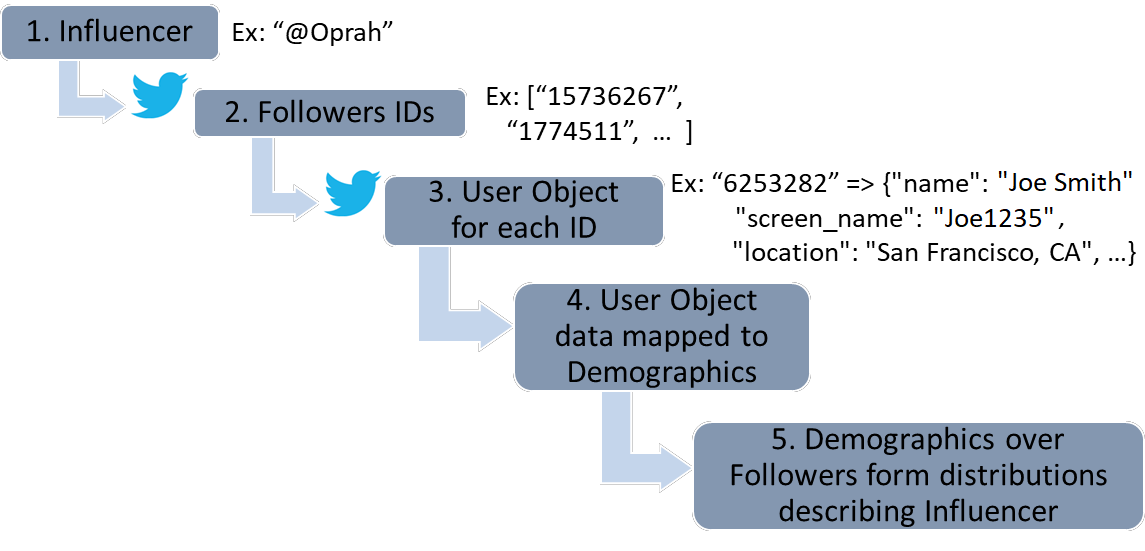
\includegraphics[width=4in]{Fig1}
\caption[Category 1 vs. Category 2 locations]{Category 1 are locations with a high accuracy where at least 75\% of users post messages with coordinates that are within 100 miles of coordinates geocoded from the self-reported location. Category 2 has low accuracy where less than 3.4\% of users match. Locations that are utilized by at least 100 users tend to be mostly Category 1.}
\label{fig_ch2_1}
\end{figure}

Fig. 2.2 (top) shows that the majority of category 1 locations get associated with a high-level location type. This is especially true as the minimum number of users that utilize location increases. For locations with number of users $\geq 100$, the high-level location type captures 99.6\% (843 out of 846) of category 1 locations. 

\begin{figure*}[htp]
\centering
   \subfloat[Category 1]{\label{fig_ch2_2a}
      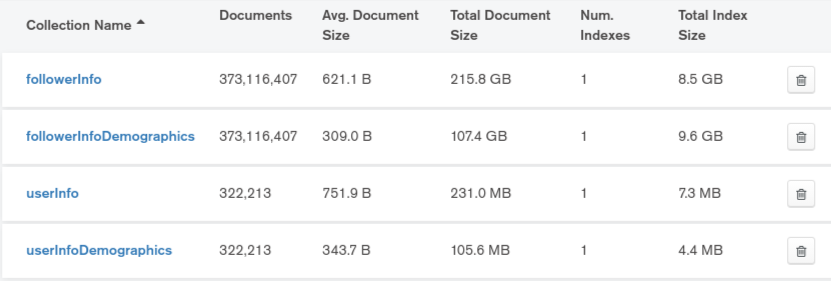
\includegraphics[width=.55\textwidth]{Fig2}}
\\
   %\hspace*{\fill}   % maximize separation between the subfigures
   \subfloat[Category 2]{\label{fig_ch2_2b}
      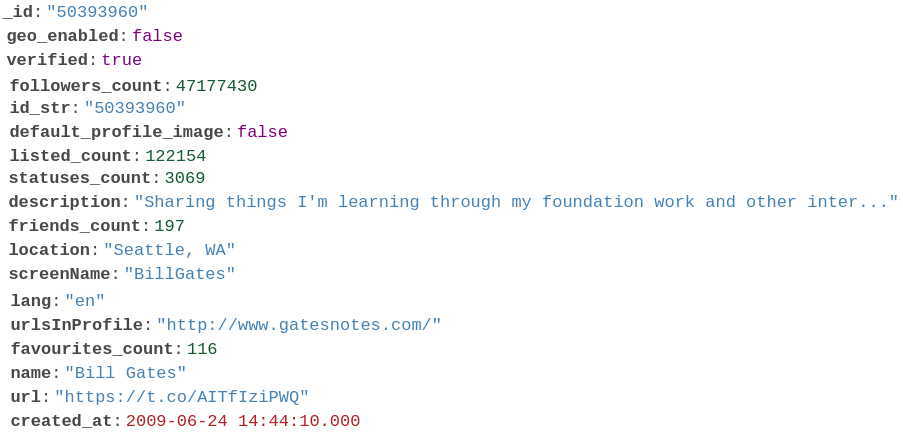
\includegraphics[width=.55\textwidth]{Fig3}}
   \caption[Category 1 vs. Category 2 (good vs. poor geocoding performance)]{\textbf{Top} --  Large ratio of Category 1 locations (good geocoding performance) associated with a high-level address. The chart confirms that majority of properly geocoded locations are not at street-level (occasionally a street-level address is proper such as when associated with an address belonging to a facility such as a University). \textbf{Bottom} --  Large ratio of Category 2 locations (those that are inaccurately geocoded) are associated with street-level. The chart confirms that street-level addresses are mostly errors.} \label{fig_ch2_2}
\end{figure*}

Conversely, Fig. 2.2 (bottom) shows inaccurately geocoded locations captured by category 2 are associated with low-level location type. The overall trend does not decrease, but the number of associated mistakes is small because the number of category 2 locations is small. For number of users $\geq 100$ per location the high-level location type captures 32.56\% (14 out of 43) of category 2 locations. Examples of locations that do get associated with a high-level location type: Midwest to Midwest WY, Nederland to Nederland CO, Nowhere to Nowhere OK, Moon to Moon PA, and others where a popular concept matches a city name. In the next section, we experiment with improving the heuristic by incorporating additional features via a classifier.

\section{Classifier}

The features that were utilized in the heuristic, as well as additional features, are utilized in a classifier. Features used in heuristic correspond to whether geocoder associates location with university, zip, or a political entity. These were the additional features tried:

\begin{itemize}
\item Text Overlap = returns percent character overlap between textual self-reported location and textual address associated by the geocoder.
\item City/State exact = returns true if tokens from the query can be combined to match city and state address component exactly, false otherwise. 
\item Populous City = for cities with a large population, we assume that city name may be known to most human users such that the state need not be spelled out. Location matched to 2016 US census data using city and state that Google associates with the query string. This rule returns true if city associated by geocoder has a population of over 50K, false otherwise.
\end{itemize}

We utilized location categories established by our approach for automatically generating labels for locations used by at least fifty users. Accurately geocoded locations (TRUE label) are those with $ACC@100$ $\geq$ 0.75 (category 1). Poorly geocoded locations (FALSE label) are those with $ACC@100$ $\leq$ 0.034 (category 2). For classifier, we considered Naïve Bayes and decision tree using gain ratio, information gain, and Chi-square interaction detector (CHAID). Each trained using 5-fold-cross-validation utilizing the RapidMiner software package. Fig. 2.3 shows the best performing classifier, a decision tree classifier using the CHAID criterion. Table 2.8 compares the performance of classifier vs. high and low location types.

\begin{figure}[!t]
\centering
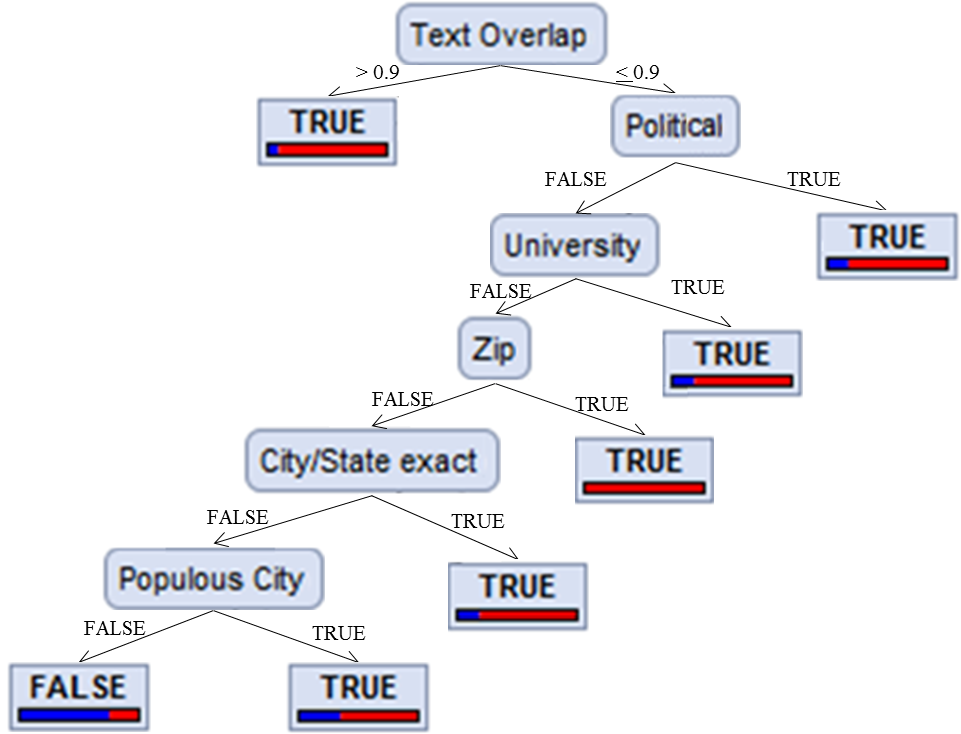
\includegraphics[width=4in]{Fig4}
\caption{Decision Tree Classifier for Geocoding}
\label{fig_ch2_4}
\end{figure}

\begin{table}
\small
\renewcommand{\arraystretch}{1.2}
\caption{Error Rate over All Users}
\label{table_ch2_8}
\centering
\begin{tabular}{|c|c|c|c|}
\hline
\bfseries Location Set & \bfseries MeanED & \bfseries MedianED & \bfseries ACC@100\\
\hline
Low level&1645.62&826.22&0.2201\\
\hline
High Level&236.75&6.29&0.803\\
\hline
Fail Classifier&1705.12&879.45&0.1969\\
\hline
Pass Classifier&237.1&6.3&0.8027\\
\hline
\end{tabular}
\end{table}

Error measures in the table were computed over all users that belong to location set vs. averaged over individual locations. The locations that fail classifier vs. low-level location type have a higher error rate across the three measures. The pass classifier vs. high-level location type shows a slight decrease. When analyzing individual locations we saw that the decision tree classifier made several improvements. For example, sometimes a popular keyword such as Mars would match a real city (category 2 type error). It is still possible to accurately geocode Mars, TX, but because it is a small city both city and state need to be specified in the self-reported location. The decision tree also captured well-formed locations that are associated with a point of interest such as Fort Knox KY being an army fort, Niagara Falls being a natural feature, and other locations that were previously missed. Otherwise, the overall performance was similar to the heuristic developed. 

The rules of the classifier illustrate that it is important to consider whether a location that is matched up by geocoder contains both the city and state as this is less ambiguous than a city name by itself. Google's geocoder is limited by the amount of API calls it can freely make daily and thus matching using a rule-based approach (using locations that contain a known city/state or city/country) is an option for a high precision/low recall solution.

\section{Conclusions}
The research has explored various types of geocoding errors and has established expected error rates for well and poorly geocoded locations in the context of Twitter. These measures can be used to decide whether the commercial off-the-shelf geocoder is performing as it should on Twitter data. For geocoder from Google, it was illustrated that a 35\% reduction in error can be achieved. 




%There are multiple choices available for geocoding a textual location: (1) utilizing an existing off the shelf geocoder, (2) developing one from scratch, or (3) customizing  combination of the two. We have illustrated that a combination of the two results in an optimal system; geocoder by itself will suffer due to out of domain strings that will lead to poor precision. Due to the complexity of the human language developing a complicated rule based approach without relying on geocoder will most likely result in poor precision and poor recall. A combination of a geocoder and rules leads to an overall 35\% reduction in error thus improving precision while maintaining high recall. If the output from geocoder is not available (since geocoder such as from Google has a maximum number of daily API calls allowed) the rules devised can be used to match on strings containing city/state or city/country (while disregarding punctuation and capitalization) will lead to a low recall but high precision and quick processing solution. 
